% IEEE standard conference template; to be used with:
%   spconf.sty  - LaTeX style file, and
%   IEEEbib.bst - IEEE bibliography style file.
% --------------------------------------------------------------------------

\documentclass[letterpaper]{article}

\usepackage 		 {algorithm	} % A suite of tools for typesetting algorithms in pseudo-code
\usepackage[noend	]{algpseudocode}
\usepackage 		 {amsmath		} % AMS mathematical facilities for LaTeX
\usepackage 		 {amssymb	} % Amsfonts + few hundred additional mathematical symbols
\usepackage[english	]{babel	    	} % Multilingual support for LaTeX
\usepackage 		 {etoolbox 		}
\usepackage 		 {graphicx 		} % Enhanced support for graphics
\usepackage 		 {hyperref 		} % Extensive support for hypertext in LaTeX
\usepackage 		 {spconf 		} % Style file for Signal Processing Society Conferences

\usepackage 		 {epstopdf		} % Convert EPS to 'encapsulated' PDF using GhostScript

\graphicspath{{figures/}} % Relative path to figure sources

\newcommand{\mypar}[1]{{\bf #1.}} % Bold paragraph titles

%%%%%%%%%%%%%%%%%%%%%%%%%%%%%%%%%%%%%%%%%%%%%%%%%%%%%%%%%%%%%%%%%%%%%%%%%
%    Custom tools for code snippets preparation in nice pseudocode
%%%%%%%%%%%%%%%%%%%%%%%%%%%%%%%%%%%%%%%%%%%%%%%%%%%%%%%%%%%%%%%%%%%%%%%%%
	\algrenewcommand\algorithmicrequire{\textbf{Input:}} % "Input" instead of "Require" in code snippet

	% begin vertical rule patch for algorithmicx (http://tex.stackexchange.com/questions/144840/vertical-loop-block-lines-in-algorithmicx-with-noend-option)
	\makeatletter
	% start with some helper code
	% This is the vertical rule that is inserted
	\newcommand*{\algrule}[1][\algorithmicindent]{\makebox[#1][l]{\hspace*{.5em}\thealgruleextra\vrule height \thealgruleheight depth \thealgruledepth}}
	% its height and depth need to be adjustable
	\newcommand*{\thealgruleextra}{}
	\newcommand*{\thealgruleheight}{.75\baselineskip}
	\newcommand*{\thealgruledepth}{.25\baselineskip}

	\newcount\ALG@printindent@tempcnta
	\def\ALG@printindent
	{
    		\ifnum \theALG@nested>0% is there anything to print
        		\ifx\ALG@text\ALG@x@notext% is this an end group without any text?
           			% do nothing
        		\else
            			\unskip
            			\addvspace{-1pt}% FUDGE to make the rules line up
           			% draw a rule for each indent level
            			\ALG@printindent@tempcnta=1
            			\loop
               				\algrule[\csname ALG@ind@\the\ALG@printindent@tempcnta\endcsname]%
                			\advance \ALG@printindent@tempcnta 1
            			\ifnum \ALG@printindent@tempcnta<\numexpr\theALG@nested+1\relax% can't do <=, so add one to RHS and use < instead
            			\repeat
        		\fi
    		\fi
	}

	% the following line injects our new indent handling code in place of the default spacing
	\patchcmd{\ALG@doentity}{\noindent\hskip\ALG@tlm}{\ALG@printindent}{}{\errmessage{failed to patch}}
	\makeatother

	% the required height and depth are set by measuring the content to be shown
	% this means that the content is processed twice
	\newbox\statebox
	\newcommand{\myState}[1]
	{
    		\setbox\statebox=\vbox{#1}%
    		\edef\thealgruleheight{\dimexpr \the\ht\statebox+1pt\relax}%
    		\edef\thealgruledepth{\dimexpr \the\dp\statebox+1pt\relax}%
    		\ifdim\thealgruleheight<.75\baselineskip
        		\def\thealgruleheight{\dimexpr .75\baselineskip+1pt\relax}%
    		\fi
    		\ifdim\thealgruledepth<.25\baselineskip
        		\def\thealgruledepth{\dimexpr .25\baselineskip+1pt\relax}%
    		\fi
		%\showboxdepth=100
		%\showboxbreadth=100
		%\showbox\statebox
		\State #1%
		%\State \usebox\statebox
		%\State \unvbox\statebox
		%reset in case the next command is not wrapped in \myState
		\def\thealgruleheight{\dimexpr .75\baselineskip+1pt\relax}%
		\def\thealgruledepth{\dimexpr .25\baselineskip+1pt\relax}%
	}
	% end vertical rule patch for algorithmicx
%%%%%%%%%%%%%%%%%%%%%%%%%%%%%%%%%%%%%%%%%%%%%%%%%%%%%%%%%%%%%%%%%%%%%%%%%


\title{Parallel Implementation of Breadth-First Search} % TODO: We need good descriptive title. This one is work version.

\name{Yauhen Klimiankou, Lukas Strebel, Stephanie Christ} 
\address{Department of Computer Science\\ ETH Z\"urich\\ Z\"urich, Switzerland}

%TODO: ~5 figures (strong scaling + weak scaling on Intel + Xeon Phi and code snippet) + ~1 table (evaluation results).

% NOTE! Please, maintain the Pretty Print style of the document source code. Keep appropriate aligning and nesting, one sentence per line and separate paragraphs by empty line!

\begin{document}
	\maketitle

	\begin{abstract} % Roughtly half a column.
		% TODO: fill at the end of writing as a brief retelling of the whole paper content.
		 
		%%| Describe in concise words what you do, why you do it (not necessarily
		%%| in this order), and the main result. The abstract has to be
		%%| self-contained and readable for a person in the general area. You
		%%| should write the abstract last.
	\end{abstract}

	\section{Introduction}\label{sec:intro} % Roughtly page + TODO:~4 references.
		A graph is one of the most powerful and widely used abstract data types, because it is convenient for the representation of a wide range of real-world objects in computer applications.
		Most graph applications and appropriate algorithms involve graph traversals, during which knowledge about the graph is updated as each vertex is visited. 
		Depth-first search (DFS) and Breadth-first search (BFS) are two basic strategies for graph traversal and searching in graphs.
		While DFS starts the graph traversal at the root and explores as far as possible along each branch before backtracking, BFS in contrast inspects all the neighbouring vertices starting from the root and then for each of those neighbour vertices in turn, it inspects their neighbour vertices which were unvisited, and so on, level by level.
		The set of vertices with the same minimal distance from the root vertex is called a level in terms of BFS.
				
		BFS is one of the most basic graph algorithms and a foundation for a wide range of more specific algorithms used for tasks such as finding all vertices within one connected component of the graph, collection copying in garbage collection algorithms, finding the shortest path between two specified vertices, testing a graph for bipartiteness, mesh numbering, computation of the maximum flow in a flow network etc.
		%BFS is a first class algorithm commonly used for solving different real-life and scientific problems on systems represented by networks. % repeats the previous sentence
		Most notable examples of its industrial applications are navigation systems for finding the shortest path between two specified destination points on a road network, finding the shortest route to a specified host in a computer network or the shortest route to a host with specified properties, web indexing performed by web crawlers used by web search engines to maintain their search database in the actual state and social interconnections investigation on the base of social networks.
		
		At this time, the information technology industry is experiencing a great shift introduced by mass migration to multi-core processors and emergence of many-core computer systems (up to 120/240 physical/logical cores in theory and 60/120 physical/logical cores in practice on Intel platform, and up to 64 physical cores on AMD platform) and coprocessors (computation accelerators) like Intel Xeon Phi (up to 61 physical cores).
		All these wide-spreading and emerging computer systems are examples of shared memory architectures (SMA).
		Wide dissemination of computer systems with shared memory architecture and trends indicating that the development of such systems is the main direction of the further performance improvement of computer systems on one hand, and the widespread use of BFS for a wide range of applications on the other hand, make the question about the most efficient and scalable variant of parallel version of BFS in the environment of such kind of systems relevant to this time.
		
		In this paper, we describe an experimental study of different variants and approaches of parallel BFS algorithms based on OpenMP for SMA computer systems and the design, implementation and evaluation of the variant with which we finally came up as the most promising.
		We refer to this variant as optimistic parallel BFS.
		According to our experimental results, it significantly outperforms all other approaches in the environments of AMD SMA platform and Intel Xeon Phi accelerator.
		Our experiments and analysis of its results highlighted that the efficiency of BFS algorithm variants heavily depend on the properties of the underlying environment (hardware platform, operating system, compiler), as well as on the properties of the graph to which it is applied.
		We conclude also that the cost of synchronization which is usually used for preserving consistency can be too high, but can in some cases be eliminated.
		
		It is important to note that the optimistic parallel BFS can't be considered as a universal optimal variant of BFS for all kinds of the SMA computer systems.
		Instead it must be considered as a source of a more general approach to the implementation of BFS for the environment of a particular kind of SMA system.
		To achieve the most optimal approach for a particular computer system, investigation of different variants of parallel BFS and the most suitable optimizations must be done for the environment of the system of interest, because our results tell us that the efficiency of BFS itself and optimizations used in it heavily depend on the target environment. 
	
	% \section{Experiments}\label{sec:expe} % Roughtly two pages - half a column. + 4 plots
	% \section{Discussion}\label{sec:disc} % Roughtly column. + ~1-2 references + 1 table
	% \section{Summary and Conclusion}\label{sec:suco} % Roughtly half a column.


	\section{Background: Breadth-first search}\label{sec:background}
	
	
	In this section, we will give a brief overview over the idea of breadth-first search and its sequential asymptotic runtime cost, as well as a short discussion of different graphs and graph properties. 
	
	
	\mypar{Breadth-first search}
	Breadth-first search (BFS) is a graph traversal algorithm which starts at a source vertex and either travels until it finds a specific vertex or until it has explored all connected vertices. 
	In the first step, all vertices adjacent to the source are explored and stored in some data structure (called frontier or next) as well as marked as visited. 
	In the second step, the newly visited vertices become the new sources (called neighbours or current) from which the search continues by repeating this step. 
	Doing a traversal this way assures that all the nodes at the same distance to the source are explored before any vertices with greater distance can be explored. 
	All the vertices in the same distance to the source are called level.
	
	The desired output of a BFS can differ depending on where it is applied. With minimal modifications BFS could deliver a predecessor map, where every vertex points to only one parent, or a distance map, where the distance to the source is stored for every vertex. Since the predecessor map is not necessarily unique, we choose to return a distance map as our output to make verification of correctness simpler.  
	
	The sequential version of a BFS can be implemented using a single queue and has a theoretical asymptotic runtime of $\mathcal{O}(\lvert V\rvert + \lvert E\rvert )$, where $\lvert V\rvert$ is the number of vertices and $\lvert E\rvert$ the number of edges in the connected graph.
	
	
	\mypar{Graphs}
	As previously mentioned graphs are a widely used abstract data type, which depending on their source and use can have widely different properties which in turn account for strong variations in the performance of BFS and other graph algorithms.
	
	To account for this we used real world graphs and specific synthetic graphs provided by the University of Florida Sparse Matrix Collection \cite{SparseMatrixCollection}, notably some graphs from the DIMACS10 challenge, in our test and experimental cases.
	The mentioned synthetic graphs are mostly so called Kronecker graphs \cite{Leskovec:2010:KGA:1756006.1756039}, which are generative network graphs that obey the main static network patterns observed in real networks.
	Especially the small-world property is worth mentioning since it provides a reasonable assumption that a given node in a network has a large enough neighbourhood so that a parallel BFS can be useful.	
	


	\section{Related work} \label{sec:rewo} % Roughtly column. + ~8 references.
		BFS is not an easy candidate for parallelisation.
		It is inherently memory intensive and has pure spacial locality which introduces significant performance loss on today's computer systems with the growing gap between CPU performance, memory performance and increasing memory latencies.
		As a result, scalability of a parallel version of BFS will be bound by the performance characteristics of the memory subsystem of the target computer system. 
		Nevertheless, intensive use of BFS in the wide range of the applications create a high interest in the most efficient and scalable versions of parallel BFS.
		As a result, a number of papers were published in this field. 
		
		Beamer et al.\cite{beamer2011searching} report a different algorithm to deal with the performance issues encountered when designing a BFS algorithm. 
		The proposed hybrid algorithm combines the usual top-down approach with a new bottom-up part. 
		In the bottom-up part, a level is processed by searching a parent for all unvisited vertices, where a parent is only valid if it is a neighbour of the unvisited vertex. 
		This is advantageous for small-world graphs because it saves accesses and data processing when a large fraction of the vertices are in the frontier. 
		To get optimal results, a hybrid algorithm is proposed where a heuristic switching criteria controls the use of top-down or bottom-up step depending on the size of the frontier and a predicted size of the next frontier. 
		Yasui et al.\cite{6691600} describe an implementation of such a hybrid algorithm for Kronecker and R-MAT graphs, as well as a detailed description of the heuristic switching parameters.
	
		Berrendorf\cite{Berrendorf:14} describes a technique to avoid atomic operations in a generalized scenario. 
		The scenario is given as an if-statement followed by some operations that change a state, where multiple threads might execute the predicate and execute the operations afterwards. 
		The operations need to change the state to the same value if executed multiple times, otherwise there exists a race condition, i.e. the change of the distance of a visited vertex to the value of the level or the addition of a vertex to the next frontier. 
		The trade-off is that doing a BFS this way can result in additional work, since any unvisited vertex may get added multiple times.
		
		%In our proposed technique we moves future at the way of avoiding atomic operations and intra-level synchronization at all.   % What do you want to say with this sentence?
		In our final proposed technique we go the way of avoiding atomic operations and synchronization within levels at all.
		The only synchronization point left in our proposed algorithm is an implicit barrier between the processing of different levels of the graph.
		
		In addition to this, we have compared a number of different approaches based on different synchronization primitives and techniques and load balancing strategies.

	
	
	\section{Design and implementation}\label{sec:deim} % Roughtly page + half a column. + 1 code snippet
		The goal of our efforts is to achieve the most efficient and scalable algorithm of parallel BFS for Shared Memory Architectures. 

		\subsection{Possible directions of performance boosting}
			There are three main directions of performance boosting in the way of making BFS parallel.
			
			\textbf{Improvement of cache utilization.}
			It is not a secret that due to the big gap between the performance of CPU subsystems and the memory subsystem performance of modern computer systems, as well as latencies of memory access, make the performance of the algorithms highly sensitive to the provided CPU cache utilization. 
			Introduction of multicore computer systems made the problem even more complex because  we are now forced to think about careful splitting of the active data set between all available processors to avoid cache misses introduced by cache lines flip-flopping. 
			Unfortunately, in the case of the BFS, we are forced to work with a data set with inherently pure spatial locality. 
			Due to this, this way of optimization was rejected.
			
			\textbf{Load balancing improvement.} 
			Goal of this approach is to achieve highest possible level of overall utilization of all available processor elements by avoiding the idle time of CPUs introduced by waiting for the arrival of a new job.
			It is one of the promising approaches, because the classical approach to BFS parallelisation relies on a sequential graph level processing where each level is processed in parallel.
			As a result, all CPUs that finished their work are forced to wait until the processing of the current level will be accomplished by other still busy processors.
			Nonetheless, this direction was rejected in favour of the synchronization avoidance. 
			
			\textbf{Avoidance of synchronization.}
			Synchronization is an expensive but necessary component of almost all parallel algorithms.
			It is expensive in both dimensions, as synchronization usually takes many CPU cycles (in absolute numbers), which reduces scalability. 	% TODO: What is meant with this sentence? Do you mean that it takes a lot of CPU cycles, and because of this reduces scalability?
			Our main design direction was figuring out of the cheapest scheme of synchronization while still providing consistency.
			Ideally, we would like to eliminate synchronization at all.
			
			

	
		% TODO
		% hybrid: doing top-down or bottum up, depending on heuristic switch. uses 1x OMP critical section in top-down part and localneighbourhoods + prefix sum to add them together at each level in the bottom-up part. Idea from paper by Yasui et al
		% nonlevel: using 1xCAS to check visited and  1xOMP critical for the distance update (needs to see if unvisited or visited from further away), frontier is a single queue. if a thread finishes with his part he waits for the others to finish (no loadbalancing). Idea from talking with Timo.
		% nonlevel with work stealing. Idea is for threads that are finished with their part to steal work from a randomly choosen other thread. Only works with too much synchronization (slow) at the moment. Idea from talking with Timo.
		
		\subsection{Different approaches}\label{sec:approaches}
		
		%Now comes the ``beef'' of the report, where you explain what you
		%did. Again, organize it in paragraphs with titles. As in every section
		%you start with a very brief overview of the section.
		%
		%In this section, structure is very important so one can follow the technical content.
		%
		%Mention and cite any external resources that you used including libraries or other code.
		
		We implemented many different algorithms and multiple variants for most of them. They return a distance map from one source vertex to all reachable vertices in the graph.
		
		All our implementations are based on OpenMP for synchronization.
		
		\mypar{Top-down}
		Most of our approaches are based on a simple top-down algorithm. 
		The idea is to do a level-synchronous traversal of the graph by keeping record of the vertices in the current as well as those in the next level (``frontier'' and ``neighbour'') in two data structures of the same type. 
		We then set the frontier to the current neighbours after each level. 
		This leads to an implicit barrier, as the threads that finish earlier have to wait on the others before proceeding to the next level.
		We experimented with different data structures and synchronization methods.
		
		% naive
		% using 1x OMP critical section (check visited and add to frontier), frontier is a vector to allow easy dynamic splitting after each level (load balancing between threads). basically naive implementation
		The naive variant of the top-down algorithm uses a global standard vector for the frontier to allow easy dynamic splitting between the threads in each level. 
		This balances the load between threads, however it has a significant overhead because it relies on a critical section (\verb+OMP critical+) for checking whether the vertices were already visited and subsequently inserting them into the neighbour data structure.
		
		% topdownCAS
		% using CAS (check visited) + OMP critical section (add to frontier), also vector frontier. Idea from paper by Berrendorf
		To improve the naive implementation, the first approach to get rid of the critical section as it produced a lot of overhead. 
		We attempted this by using an atomic, the built-in \verb+__sync_val_compare_and_swap+ (CAS), to atomically check whether a vertex was visited and setting the correct distance. 
		In addition to the atomic, this variant uses a local neighbourhood data structure (standard vector) to be able to do without a critical section. 
		Only at the end of each level a lock (\verb+omp_lock_t+) is needed to combine the local neighbourhoods to a global one, which can then be distributed between the threads for the next level. 
		This is an idea adapted from Berrendorf \cite{Berrendorf:14}.
		
		% topdown_ifCAS
		% same as topdownCAS but doing a nonatomic visited check before each CAS, Idea from paper by Berrendorf
		An extended version of the algorithm before does a non-atomic check if a vertex visited before each CAS. 
		This lets us treat the cases where the vertex had already been visited without any synchronization.
		
		% maybe better leave this method out, as it is fairly similar to the optimistic approach. The only difference lies in the data structures used.
		%
		% topdown_nonatomic
		% doing the visited check nonatomic (adds additional work but no race condition), using localneighbourhood and OMP lock to add them to the global neighbourhood after a thread has looked at all neighbours from one node. Idea from paper by Berrendorf
	%	Also inspired by Berrendorf \cite{Berrendorf:14} is the idea to remove atomics altogether. 
	%	This results in a race condition where additional work for the next level is created, as some vertices might be added to the neighbours multiple times. 
	%	However, expensive atomics are omitted, which results in a trade-off between the additional time from the added work and the faster runtime by leaving out the CAS. 
	%	This algorithm still uses a local neighbourhood and a lock when combining them.
		
		
		% tbb_parallelqueue
		% doing a top-down method using 1x OMP single for level synchronization and TBB concurrentqueue as a concurrent frontier

		% even_odd_parallelqueue
		% using only implicit OMP barrier for level synchronization. switching between two TBB parallelqueue frontiers			
		To compare all synchronisation approaches we also looked into concurrent data structures to solve the synchronisation problem of the algorithm i.e. a concurrent queue to handle the neighbour and frontier queue.
		The design and implementation of such a data structure is a subject of its own and beyond the scope of this paper. Therefore instead of focusing on designing or implementing such a concurrent queue we used the one implemented in the Intel Threading Building Blocks library (Intel TBB version 4.3).
		We found that using two concurrent queues for the neighbour and frontier and swapping them between levels in the same way as in the above mentioned implementations diminishes the time saved by not using explicit synchronisation significantly.
		To perform better we implemented a version that uses two concurrent queues that instead of swapping just switch roles from frontier to neighbour and vice versa after each level.
		This way the swapping in the serial part of the implementation is replaced by a few if-statements while essentially doing the same algorithm.
		 
		
			
		\subsection{Optimistic BFS algorithm design}
			Our proposed algorithm was designed for the environment of OpenMP and due to this employs data-parallelism approach. 
			It accepts two input parameters: the graph description and the index of the root node.
			The graph description is a list of lists, in which each top-level list denotes one of the graph vertices and the bottom level list enumerates all neighbours of the appropriate vertex, thus denoting all edges connected to it.
			The algorithm returns a distance map for the specified root node.
			
			The core of the proposed algorithm is classical. 
			It is a level by level sequential top-down walking through the graph, where in each iteration we discover all unvisited neighbours of the vertices in the current level.
			
			One of the core design decision related to memory management.
			Classical approach employs dynamic data structures like lists and queues which are used for level member nodes.
			This approach is purely suitable for efficient parallelism, because it explicitly introduce synchronization point and can introduce implicit synchronization point via memory chunks allocation/deallocation. 
			Instead we propose to use raw memory chunks allocated and freed only once in the prologue and epilogue of the algorithm.
			Our approach utilize $4 \cdot number\_of\_the\_node$ bytes of memory allocated in 4 equal chunks:
			\begin{enumerate}
				\item Flags array tracking visited nodes.
				\item Flags array holding all nodes of the current level.
				\item Flags array used for tracking of the next level nodes.
				\item Flags array used for resetting.
			\end{enumerate}
			
			After the end of each level processing the last three flag arrays exchange they roles by simple and efficient pointers swapping in accordance with the next rotation scheme: current level $\to$ resetting $\to$ next level $\to$ current level.
			As a result each level processing started with set of current level nodes collected during previous level processing and clear map of next level nodes. 

			Byte per node memory allocation scheme was chosen instead of classical bit masks because it allows to simplify memory access patterns and eliminate synchronization which would be required otherwise.
			Bit mask update via OR operation includes two elementary memory access operations, because this operation is an example of read-modify-write operation.
			As a result it introduces source of inconsistency in the concurrent environment.
			This consistency can be easily fixed by using of the lock prefix (atomic operations on Linux and interlocked operations on Windows), but this will mean one more point of synchronization which we are trying to eliminate.
			
			Level processing performs in parallel using for cycle of the OpenMP.
			This cycle introduce the only synchronization point of the proposed algorithm via implicit barrier at the end of cycle.
			
			Each iteration of the parallel for cycle containst two conditional actions: making a step on the graph walking and clearing of the clearing flags array.
			Last one action is made only by threads processing the node at the start of the cache line and clear whole cache line at once.
			This policy reduces the level of false cache sharing. 
			Stepping through the graph performs only for nodes specified by the flags array of the current level of the walking.
			For such nodes algorithm algorithm updates the distance map, flags array of visited nodes and flags array for the next level of all unvisited neighbor nodes .
						
			\begin{algorithm}
				\caption{Optimistic BFS}
				\label{alg:optbfs}
				\begin{algorithmic}[1]
					\Require
						\Statex Adjacency list: $AF = \lbrace AF_k \rbrace$
						\Statex Source node: $s$
						\Statex Reference to distance map: $distance = \lbrace distance_k \rbrace$
					\Statex

					\State $n \gets$ size ($AF$) \Comment{Number of vertices}					
					
					\State $currLevel_k \gets$ False, $\forall k \in n$
					\State $nextLevel_k \gets$ False, $\forall k \in n$
					\State $visited_k \gets$ False, $\forall k \in n$
					\Statex
					
					\State $currLevel_s \gets$ True
					\State $visited_s \gets$ False
					\State $distance_s \gets$ 0
					\Statex
					
					\State $stop \gets$ False
					\Statex
					
					\While{ $stop = $ False }
						\State $stop\gets$ True
						\ForAll{ $v \in V$ } \textbf{in parallel}
							\If{ $currLevel_v =$ True }
								\State $currLevel_v \gets$ False
								\ForAll{ $w \in AF_v$ }
									\If{ $visited_w =$ False }
										\State $distance_w \gets distance_v + 1$
										\State $nextLevel_w \gets$ True
										\State $visited_w \gets$ True
										\State $stop \gets$ False
									\EndIf
								\EndFor
							\EndIf
						\EndFor
						
						\vspace{-0.051cm} % fix issue with space in vertical bar
						
						\State swap ($currLevel$, $nextLevel$)
						\State $nextLevel_k \gets$ False, $\forall k\in n$
					\EndWhile
				\end{algorithmic}
			\end{algorithm}



						
			
%	\section{Background: Breadth-first search}\label{sec:background}
%	
%	
%	In this section, we will give a brief overview over the idea of breadth-first search and its sequential asymptotic runtime cost, as well as a short discussion of different graphs and graph properties. 
%	
%	
%	\mypar{Breadth-first search}
%	Breadth-first search (BFS) is a graph traversal algorithm which starts at a source vertex and either travels until it finds a specific vertex or until it has explored all connected vertices. 
%	In the first step, all vertices adjacent to the source are explored and stored in some data structure (called frontier or next) as well as marked as visited. 
%	In the second step, the newly visited vertices become the new sources (called neighbours or current) from which the search continues by repeating this step. 
%	Doing a traversal this way assures that all the nodes at the same distance to the source are explored before any vertices with greater distance can be explored. 
%	All the vertices in the same distance to the source are called level.
%	
%	The desired output of a BFS can differ depending on where it is applied. With minimal modifications BFS could deliver a predecessor map, where every vertex points to only one parent, or a distance map, where the distance to the source is stored for every vertex. Since the predecessor map is not necessarily unique, we choose to return a distance map as our output to make verification of correctness simpler.  
%	
%	The sequential version of a BFS can be implemented using a single queue and has a theoretical asymptotic runtime of $\mathcal{O}(\lvert V\rvert + \lvert E\rvert )$, where $\lvert V\rvert$ is the number of vertices and $\lvert E\rvert$ the number of edges in the connected graph.
%	
%	
%	\mypar{Graphs}
%	As previously mentioned graphs are a widely used abstract data type, which depending on their source and use can have widely different properties which in turn account for strong variations in the performance of BFS and other graph algorithms.
%	
%	To account for this we used real world graphs and specific synthetic graphs provided by the University of Florida Sparse Matrix Collection \cite{SparseMatrixCollection}, notably some graphs from the DIMACS10 challenge, in our test and experimental cases.
%	The mentioned synthetic graphs are mostly so called Kronecker graphs \cite{Leskovec:2010:KGA:1756006.1756039}, which are generative network graphs that obey the main static network patterns observed in real networks.
%	Especially the small-world property is worth mentioning since it provides a reasonable assumption that a given node in a network has a large enough neighbourhood so that a parallel BFS can be useful.


	
	
	\section{Experimental Results}\label{sec:exp}
	
%	Here you evaluate your work using experiments. You start again with a
%	very short summary of the section. The typical structure follows.
	
	\mypar{Experimental setup}
	%Specify the platform (processor, frequency, maybe OS, maybe cache sizes)
	%as well as the compiler, version, and flags used. If your work is about performance, 
	%I strongly recommend that you play with optimization flags and consider also icc for additional potential speedup.
	%
	%Then explain what kind of benchmarks you ran. The idea is to give enough information so the experiments are reproducible by somebody else on his or her code.
	%For sorting you would talk about the input sizes. For a tool that performs NUMA optimization, you would specify the programs you ran.
	We run experiments on three different platforms.
	
	The first platform is the EULER cluster which is operated by the HPC Group of ETH. 
	We had access to one node with a 12-core Intel Xeon E5-2697v2 processors (2.7 GHz nominal, 3.0-3.5 GHz peak). 
	As it supports hyper-threading, we ran our algorithms with up to 24 threads. 
	On this platform, we used the gcc compiler with the -O2 flag.
	
	We also ran our algorithms on an Intel Xeon Phi with 61 cores. On this platform, we used the Intel icc compiler, with the -O2 flag as well.
	
	The last platform is an AMD FX-8350 (4GHz x8, 8Gb, W2k3).
	
	% TODO
	\mypar{Results}
%	Next divide the experiments into classes, one paragraph for each. In each class of experiments you typically pursue one questions that then is answered by a suitable plot or plots. For example, first you may want to investigate the performance behavior with changing input size, then how your code compares to external benchmarks.
%	
%	For some tips on benchmarking including how to create a decent viewgraph see pages 22--27 in
	
	
	
%	{\bf Comments:}
%	\begin{itemize}
%	\item Create very readable, attractive plots (do 1 column, not 2 column plots
%	for this report) with readable font size. However, the font size should also not be too large; typically it is smaller than the text font size.
%	An example is in Fig.~\ref{fftperf} (of course you can have a different style).
%	\item Every plot answers a question. You state this question and extract the
%	answer from the plot in its discussion.
%	\item Every plot should be referenced and discussed.
%	\end{itemize}
%	
%	\begin{figure}\centering
%	  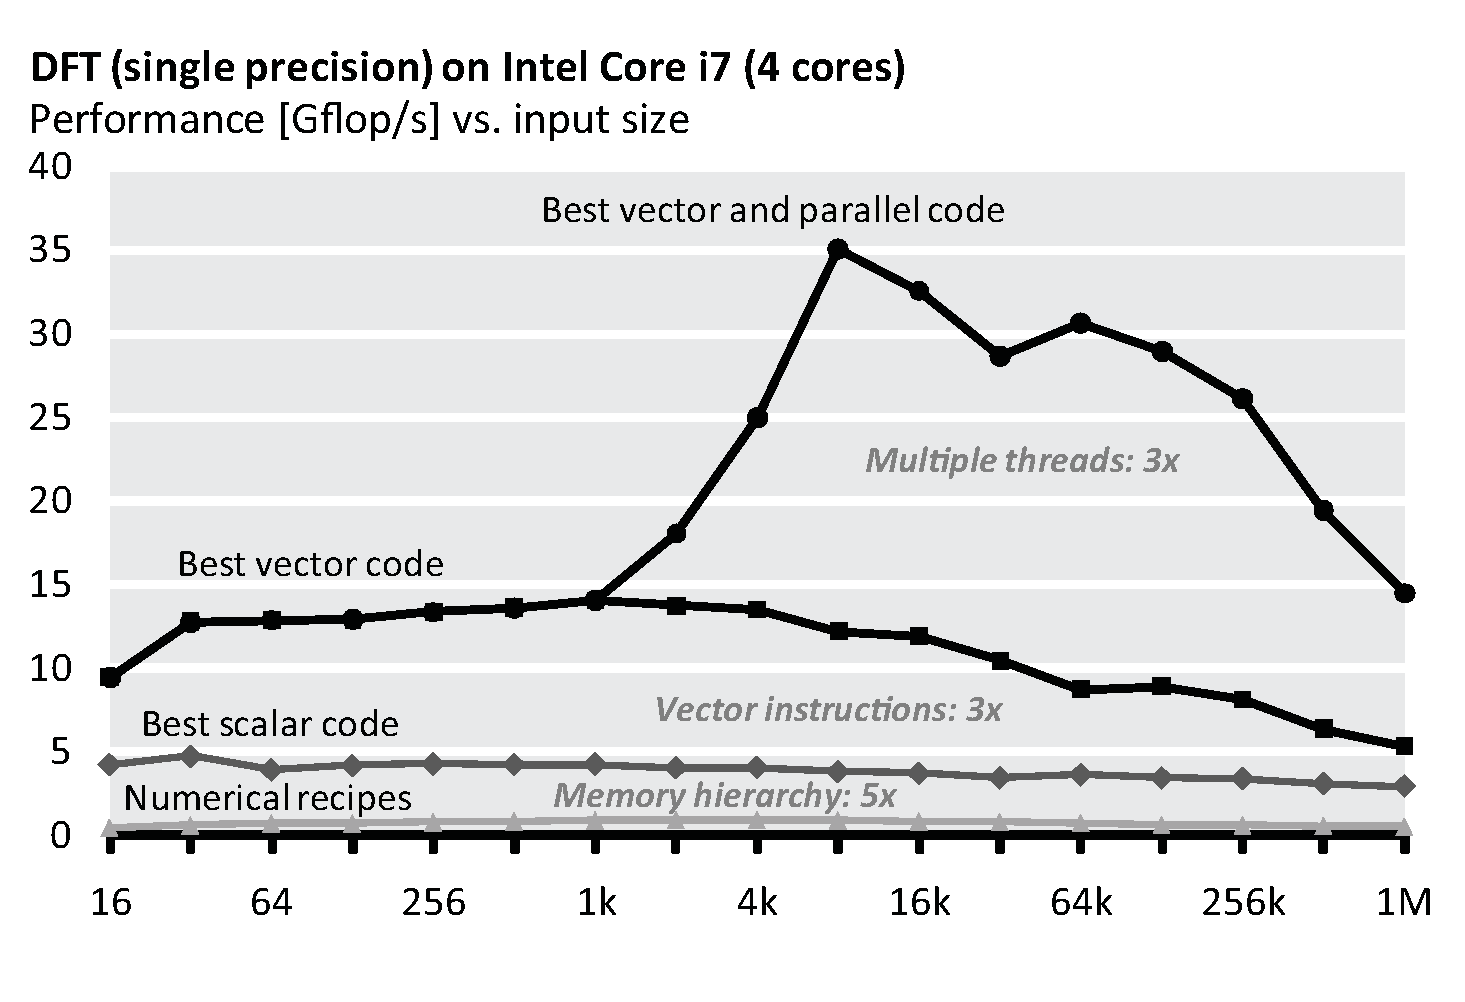
\includegraphics[scale=0.33]{dft-performance.eps}
%	  \caption{Performance of four single precision implementations of the
%	  discrete Fourier transform. The operations count is roughly the
%	  same. The labels in this plot are maybe a little bit too small.\label{fftperf}}
%	\end{figure}
	
	
	
	% TODO
	\section{Conclusions}
	
%	Here you need to summarize what you did and why this is
%	important. {\em Do not take the abstract} and put it in the past
%	tense. Remember, now the reader has (hopefully) read the report, so it
%	is a very different situation from the abstract. Try to highlight
%	important results and say the things you really want to get across
%	such as high-level statements (e.g., we believe that .... is the right
%	approach to .... Even though we only considered x, the
%	.... technique should be applicable ....) You can also formulate next
%	steps if you want. Be brief. After the conclusions there are only the references.
	
	
	
%	% TODO
%	\section{Further comments}
%	
%	Here we provide some further tips.
%	
%	\mypar{Further general guidelines}
%	
%	\begin{itemize}
%	\item For short papers, to save space, I use paragraph titles instead of
%	subsections, as shown in the introduction.
%	
%	\item It is generally a good idea to break sections into such smaller
%	units for readability and since it helps you to (visually) structure the story.
%	
%	\item The above section titles should be adapted to more precisely
%	reflect what you do.
%	
%	\item Each section should be started with a very
%	short summary of what the reader can expect in this section. Nothing
%	more awkward as when the story starts and one does not know what the
%	direction is or the goal.
%	
%	\item Make sure you define every acronym you use, no matter how
%	convinced you are the reader knows it.
%	
%	\item Always spell-check before you submit (to us in this case).
%	
%	\item Be picky. When writing a paper you should always strive for very
%	high quality. Many people may read it and the quality makes a big difference.
%	In this class, the quality is part of the grade.
%	
%	\item Books helping you to write better:
%	
%	\item Conversion to pdf (latex users only): 
%	
%	dvips -o conference.ps -t letter -Ppdf -G0 conference.dvi
%	
%	and then
%	
%	ps2pdf conference.ps
%	\end{itemize}
%	
%	\mypar{Graphics} For plots that are not images {\em never} generate the bitmap formats
%	jpeg, gif, bmp, tif. Use eps, which means encapsulate postscript. It is
%	scalable since it is a vector graphic description of your graph. E.g.,
%	from Matlab, you can export to eps.
%	
%	The format pdf is also fine for plots (you need pdflatex then), but only if the plot was never before in the format 
%	jpeg, gif, bmp, tif.


	\bibliographystyle 	{IEEEbib} % Roughtly column. (10-15 references).
	\bibliography 		{bibl_conf}
\end{document}

